\documentclass[journal]{IEEEtran}
\usepackage{amsmath,amsfonts}
\usepackage{amsmath}
\usepackage{tikz}
\usetikzlibrary{arrows.meta}
\usetikzlibrary{angles,quotes}

\begin{document}

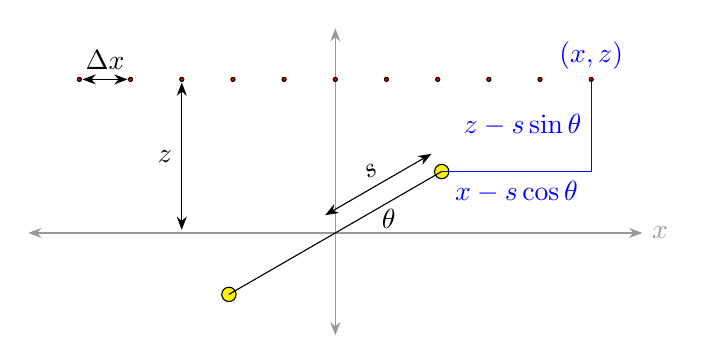
\begin{tikzpicture}[scale=1.3,>=Stealth]
  \draw[thin,<->,gray!80] (-3,0) -- (3,0) node [right] {$x$};
  \draw[thin,<->,gray!80] (0,-1) -- (0,2);
  \draw[<->] (-1.5,.03) -- node [left]{$z$} (-1.5,1.47);
  \draw[<->] (-2.47,1.5) -- node[above] {$\Delta x$} (-2.03,1.5);
  \foreach \x in {-2.5,-2,...,2.5} \draw[fill=red] (\x,1.5) circle(.02);
  \draw[fill=yellow] (30:-1.2) circle(.07) -- (30:1.2) circle(.07);
  \draw (15:.54) node {$\theta$};
  \draw[<->] (120:.2) -- node[above,sloped] {$s$} +(30:1.2);
  \draw[blue] (30:1.2) -- node[below]{$x-s\cos\theta$}(2.5,1.5 |- 30:1.2) --
  node[left]{$z-s\sin\theta$} (2.5,1.5) node[anchor=south] {$(x,z)$};
\end{tikzpicture}

\end{document}